%; whizzy chapter
% -initex iniptex -latex platex -format platex -bibtex jbibtex -fmt fmt
% 以上 whizzytex を使用する場合の設定。

%     Tokyo Debian Meeting resources
%     Copyright (C) 2010 Junichi Uekawa

%     This program is free software; you can redistribute it and/or modify
%     it under the terms of the GNU General Public License as published by
%     the Free Software Foundation; either version 2 of the License, or
%     (at your option) any later version.

%     This program is distributed in the hope that it will be useful,
%     but WITHOUT ANY WARRANTY; without even the implied warranty of
%     MERCHANTABILITY or FITNESS FOR A PARTICULAR PURPOSE.  See the
%     GNU General Public License for more details.

%     You should have received a copy of the GNU General Public License
%     along with this program; if not, write to the Free Software
%     Foundation, Inc., 51 Franklin St, Fifth Floor, Boston, MA  02110-1301 USA

%  preview (shell-command (concat "evince " (replace-regexp-in-string "tex$" "pdf"(buffer-file-name)) "&"))
% 画像ファイルを処理するためにはebbを利用してboundingboxを作成。
%(shell-command "cd image201012; ebb *.jpg")

%%ここからヘッダ開始。

\documentclass[mingoth,a4paper]{jsarticle}
\usepackage{monthlyreport}

% 日付を定義する、毎月変わります。
\newcommand{\debmtgyear}{2010}
\newcommand{\debmtgmonth}{12}
\newcommand{\debmtgdate}{18}
% (+ (* (- 2010 2005) 12) 10) started from zero
\newcommand{\debmtgnumber}{71}

\begin{document}

\begin{titlepage}
\thispagestyle{empty}
% タイトルページ:編集必要な部分は最初のマクロに飛ばすこと

\vspace*{-2cm}
第\debmtgnumber{}回 東京エリア Debian 勉強会資料\\
\hspace*{-2cm}
\includegraphics[width=210mm]{image201003/debsen.eps}\\
\hfill{}\debmtgyear{}年\debmtgmonth{}月\debmtgdate{}日

% ここはアップデートすること
\rotatebox{10}{\fontsize{32}{32} {\gt 特集1: CACert入門}}

\rotatebox{10}{\fontsize{32}{32} {\gt 特集2: 俺のlibsaneが火を噴くぜ!}}

\vspace*{-2cm}
\hfill{}
\includegraphics[height=6cm]{image200502/openlogo-nd.eps}
\end{titlepage}

\dancersection{Introduction}{上川 純一}

\begin{multicols}{2}
 

 今月のDebian勉強会へようこそ。これからDebianの世界にあしを踏み入れると
 いう方も、すでにどっぷりとつかっているという方も、月に一回Debianについ
 て語りませんか?

 Debian勉強会の目的は下記です。

 \begin{itemize}
 \item \underline{Debian Developer} (開発者)の育成。
 \item 日本語での「\underline{開発に関する情報}」を整理してまとめ、アップデートする。
 \item \underline{場}の提供。
 \begin{itemize}
  \item 普段ばらばらな場所にいる人々が face-to-face で出会える場を提供
	する。
  \item Debian のためになることを語る場を提供する。
  \item Debianについて語る場を提供する。
 \end{itemize}
 \end{itemize}		

 Debianの勉強会ということで究極的には参加者全員がDebian Packageをがりがり
 と作るスーパーハッカーになった姿を妄想しています。情報の共有・活用を通し
 て Debianの今後の能動的な展開への土台として、「場」としての空間を提供す
 るのが目的です。

\end{multicols}

\newpage

\begin{minipage}[b]{0.2\hsize}
 \definecolor{titleback}{gray}{0.9}
 \colorbox{titleback}{\rotatebox{90}{\fontsize{80}{80} {\gt デビアン勉強会} }}
\end{minipage}
\begin{minipage}[b]{0.8\hsize}
\hrule
\vspace{2mm}
\hrule
\begin{multicols}{2}
\tableofcontents
\end{multicols}
\vspace{2mm}
\hrule
\end{minipage}

\dancersection{事前課題}{上川 純一}

今回の事前課題は以下です:
\begin{itemize}
 \item 「2010年を振り返って自分がDebianでやったこと・Debian界隈でおきたこと。2011年におきると予想すること、自分がやりたいこと。」
\end{itemize}
この課題に対して提出いただいた内容は以下です。
\begin{multicols}{2}
{\small
 \begin{prework}{ matsuu }

やったこと・おきたこと
\begin{itemize}
 \item Debian勉強会に参加するようになった。
 \item VPSでDebianを使い始めた。
 \item Debianのパッケージを参考にGentooパッケージを作った。
\end{itemize}
予想・やりたいこと
\begin{itemize}
 \item DebianとGentooは徐々に衰退していき、ALL YOUR DISTRIBUTION ARE
       BELONG TO CHROMEOS.
\end{itemize}
\end{prework}

\begin{prework}{ あらきやすひろ }

予想
\begin{itemize}
 \item 無事リリースされることによるDebian派生ディストロの大崩壊と回帰。
\end{itemize}
やりたいこと
\begin{itemize}
 \item Debianで仕事!
\end{itemize}
\end{prework}

\begin{prework}{ koedoyoshida }

やったこと
\begin{itemize}
 \item ddtssでレビュー(最近お休み中)
 \item 関西KOFでの関西Debianブースのお留守番
 \item 夏冬のイベントでの書籍の頒布
\end{itemize}
おきたこと
 \begin{itemize}
  \item Squeeze freeze
\end{itemize}
予想
\begin{itemize}
 \item  Squeeze release?
\end{itemize}
やりたいこと
\begin{itemize}
 \item 予定は未定
\end{itemize}
\end{prework}

\begin{prework}{ キタハラ }

やったこと
\begin{itemize}
\item 今年は一番何もしていない年ではないだろうか?ネットサーフィン用寝床PCも死んだままだし。
\end{itemize}
やりたいこと
\begin{itemize}
\item 来年はこれを復活し、あと会社にDebianマシンを復活させたいですね。
\end{itemize}
\end{prework}

\begin{prework}{ yamamoto }

やったこと
\begin{itemize}
 \item なんかポチポチと勝手に ppc64 ポートを、マズいラーメン屋の頑固オヤ
       ジのごとく、細く長く続けていた。
\end{itemize}
おきたこと
\begin{itemize}
 \item debian-ports に、sparc64 やら powerpcspe やら armhf やらがいきな
       り現れて、いっきに抜かれて行った。
\end{itemize}
予想
\begin{itemize}
 \item 次は arm64 かな?
\end{itemize}
やりたいこと
\begin{itemize}
 \item 頑固オヤジの迷惑なラーメンを、ひたすら生み出していく。
 \item arm64 ポートに参加できるといいな。
\end{itemize}
\end{prework}

\begin{prework}{ 本庄 }

やったこと
\begin{itemize}
\item 温泉行きました。
\end{itemize}
やりたいこと
\begin{itemize}
\item また行きたいです。
\end{itemize}
\end{prework}

\begin{prework}{ yyuu }

私事ではありますが、2009 年くらいから仕事で Debian を使えるようになりま
 した。2010 年はその環境の整備に費やしているうちにあっという間に過ぎてし
 まいました。

やったこと
\begin{itemize}
 \item lenny のシステムを 100 台以上の単位で扱うことができた
 \item 自分で個人的な apt のレポジトリを作って運用できるようになった
\end{itemize}
おきたこと
\begin{itemize}
 \item 特に思いつきませんでした...
\end{itemize}

予想
 \begin{itemize}
  \item squeeze がリリースされる (2010年?)
 \end{itemize}
やりたいこと
\begin{itemize}
 \item 一部の既存ホストを lenny から squeeze へ移行したい
 \item 新興プロジェクトの Debian パッケージ化にできるだけコミットしてい
       きたい。今年は Apache Thrift などにパッチを提供できたが、今後はも
       う少し手を広げたい
\end{itemize}
\end{prework}

\begin{prework}{ 野島 貴英 }

やったこと
\begin{itemize}
 \item debian-sidのKVM上でOpensolarisを稼働させた事。
 \item debian-sidの様々なソースコードいっぱい読んだこと。
       \footnote{\url{http://d.hatena.ne.jp/nozzy123nozzy/}}
\end{itemize}
予想
\begin{itemize}
\item いわゆる携帯型tabletPC等へdebian-sidを搭載するHackがそこいら中で起きる。
\end{itemize}
やりたいこと
\begin{itemize}
 \item Contribution \& Hack!Hack!Hack!(ソフトもハードも)
\end{itemize}
\end{prework}

\begin{prework}{ henrich }

やったこと
\begin{itemize}
 \item 5月: NMプロセスを進めてDDになった
 \item 7月: スイスからDebian傘買ってみた :)
 \item 8月: Debconf に参加した
 \item パッケージのアップデートを大体継続できた
 \item その他国内のイベントに参加した
 \item RC バグ潰しに参加した
 \item 多少ではあるが翻訳作業に参加した
 \item 手が付いていないことは以下
       \begin{itemize}
	\item netbeans のパッケージ
	\item eclipse-l10n のパッケージ(ソースを見つけられない…)
	\item Knoppix-Math を Debian ベースに誘う
	\item lenny インストール記事を JP ページに載せる
       \end{itemize}
\end{itemize}
やりたいこと
\begin{itemize}
 \item 開発者リファレンス訳の完了
 \item 初歩のプログラミングができるように(pythonあたり)
 \item debconf で何かしらの成果を出せるように事前準備
 \item l10n をもっと進められるようにもっとステップと成果を明確にしたい
\end{itemize}
\end{prework}

\begin{prework}{ 岩松 信洋 }

やったこと
\begin{itemize}
 \item 組み込み関係のサポート。
 \item SH4のemdebianサポート。
 \item Macbook 関係のサポート。
 \item DDになってからの始めてのリリース作業。
 \item Debconf への参加
\end{itemize}
おきたこと
\begin{itemize}
 \item Non-packaging contributors
 \item backports が正式サービスになった。 
 \item Squeeze フリーズ
 \item Miniconf が多く行われた。
 \item fjp の急逝
\end{itemize}
予想
\begin{itemize}
 \item Debian では SH4 unstable 入り
 \item 4G ネットワークがじわじわと浸透
 \item Android を使ったタブレットデバイス祭り
\end{itemize}
やりたいこと
\begin{itemize}
 \item web 系の開発
 \item 関数型言語の習得
\end{itemize}
\end{prework}

\begin{prework}{ 野首 }

2010年はほとんど何もしませんでした...
さすがにsqueezeは2011年にはリリースされていると思いたい。
\end{prework}

\begin{prework}{ まえだこうへい }

やったこと
\begin{itemize}
 \item Debian勉強会の運営(いつもどおり)
 \item 山田さんのJPへの勧誘・加入(よくやった)
 \item 他の勉強会での勧誘(Webアプリ開発者に交友関係は増えたがDebianへの
       直接的な成果はなし)
\end{itemize}
おきたこと(予想?)
\begin{itemize}
 \item SqueezeにはCouchDB 1.0.1が入らなさそう。
\end{itemize}
やりたいこと
\begin{itemize}
 \item いろいろpendingなものを再開する。
\end{itemize}
\end{prework}

\begin{prework}{ 上川純一 }

やったこと
\begin{itemize}
 \item 子供がうまれた、Debian活動レベルが低下した。
 \item 携帯電話はAndroid携帯電話がメインになって、パソコンをあまり起動し
       なくなった。
 \item 勉強会にくるようなメンバーで、Smart Phone (iPhone or Android)をもっ
       ていない人に出会わなくなってきた。
\end{itemize}
予想
\begin{itemize}
 \item さらなるスマートフォンとタブレットの普及とそれに伴うより自由で便
       利な環境への渇望。
 \item Debianとしてはその環境との相互運用性の向上と、そのデバイス自体で
       動くシステムとしてのすすみかたが二つ考えられる。
\end{itemize}
やりたいこと
\begin{itemize}
 \item 相互運用性は少なくとも向上したいと考えている。
\end{itemize}
\end{prework}


}
\end{multicols}

\dancersection{最近のDebian関連のミーティング報告}{上川純一}
\subsection{東京エリアDebian勉強会70回目報告}

% (query-replace-regexp "<.*?>" "")
% (query-replace-regexp "^[	 ]\+" "")

東京エリアDebian勉強会。
参加者は、やまださん、前田さん、上川、野島さん、服部さん、キタハラさん、emasakaさん、matoharaさん、鈴木さん、吉田@板橋さん、高橋斉大さん、荒木(靖)さん、本庄さん、やまもとさん、吉野さんの15人でした。

ファイルシステムについてかたりました

まず最初に上川がext4について紹介しました。

nilfs について紹介しました。

btrfs について紹介しました。

ceph について紹介しました。

\dancersection{Debian Trivia Quiz}{上川 純一}

ところで、みなさん Debian 関連の話題においついていますか?Debian関連の話
題はメーリングリストをよんでいると追跡できます。ただよんでいるだけではは
りあいがないので、理解度のテストをします。特に一人だけでは意味がわからな
いところもあるかも知れません。みんなで一緒に読んでみましょう。

今回の出題範囲は\url{debian-devel-announce@lists.debian.org} や \url{debian-devel@lists.debian.org}に投稿された
内容とDebian Project Newsからです。

\begin{multicols}{2}
 %; whizzy-master ../debianmeetingresume200906.tex
% $B0J>e$N@_Dj$r$7$F$$$k$?$a!"$3$N%U%!%$%k$G(B M-x whizzytex $B$9$k$H!"(Bwhizzytex$B$,MxMQ$G$-$^$9!#(B
%
% $B$A$J$_$K!"%/%$%:$OJL%V%i%s%A$G:n@.$7!"$N$A$K%^!<%8$7$^$9!#5U$K%^!<%8$7(B
% $B$J$$$h$&$K$7$^$7$g$&!#(B
% (shell-command "git checkout quiz-prepare")

\santaku
{DACA $B$C$F$J$s$G$9$+(B?}
{Debian Admin Coaching Association}
{Debian $B$r;H$&$H(B (A)$B$"$N;R$H(B (C)$B%/%j%9%^%9$K(B (A)$B%"%l$,$G$-$k$+$b$7$l$J$$(B}
{Debian's Automated Code Analysi project}
{C}

\santaku
{DebConf11 $B$O$$$D3+:E$5$l$k$G$7$g$&(B}
{2011/6/24 - 30}
{2011/7/24 - 30}
{2011/8/24 - 30}
{B}

\santaku
{squeeze $B$N(B Linux $B%+!<%M%k$O0lL#0c$$$^$9!#2?$,0c$&$G$7$g$&!#(B}
{non-free firmware $B$rGS=|$7$?(B}
{Tux $B$/$s$rGS=|$7$?(B}
{$B0l$D$N%+!<%M%k%$%a!<%8$G(BkFreeBSD$B$H(BLinux$B$rDs6!$7$^$9(B}
{A}

\santaku
{2010/12/17 $B$N;~E@$G(BRC$B%O%0$O$$$/$D$"$k$G$7$g$&!#(B}
{3} 
{83}
{183}
{C}

\santaku
{New Maintianer $B%U%m%s%H%G%9%/$KDI2C$5$l$?%a%s%P!<$O!)(B}
{Xavier Oswald}
{Enrico Zini}
{Kenshi Muto}
{A}


\end{multicols}


%-------------------------------------------------------------------------------
\dancersection{2010年の東京エリアDebian勉強会をふりかえって}{上川 純一}
%-------------------------------------------------------------------------------
\index{debianjp@Debian JP} 
\index{とうきょうえりあ@東京エリアDebian勉強会}
\index{2010ねん@2010年}

今月で6年目のDebian勉強会が終了しました。
Debian Developer の数も着々と増えていき、当初の目標が達成されてきていま
すね。

今年東京エリアDebian勉強会常連のやまねさんがDebian Developerになりました。
苦節6年おめでとうございます。
% ueno ? kiwamu ?

Debian Maintainer 申請も複数通りました。
% FIXME: だれが今年通ったか?

\subsection{基本的な数値}

Debian 勉強会は毎回事前課題事後課題を設定しており、予習復習を必要だとう
たっている勉強会です。
実際にどれくらいの人が出席しているのか、またその人たちがどれくらい事前課
題・事後課題を提出しているのか、確認してみましょう。
\fgref{fig:attendandprepostwork}です。
値は一年の移動平均です。

結果を見ると事前課題の提出率が2009年に低下傾向にあったのが、2010年に反転
上昇しています。これはDebian勉強会予約システムの導入により事前課題の提出
が簡単になったことと関係ありそうです。また、別の傾向として事後課題(ブロ
グ)の率が低下傾向にあります。もうブログは流行らないのかもしれません。

\begin{figure}[ht]
 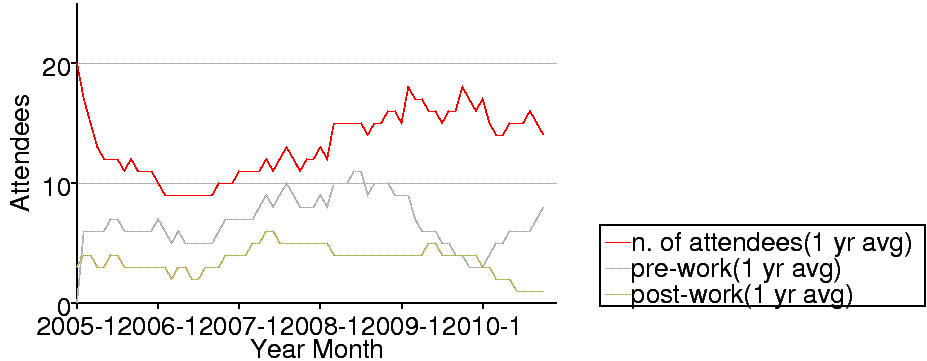
\includegraphics[width=0.5\hsize]{image201012/memberanalysis/attend.png}
\caption{東京エリアDebian勉強会事前課題・事後課題提出実績(12ヶ月移動平均)}\label{fig:attendandprepostwork}
\end{figure}

毎回の参加者の人数と、その際のトピックを見てみます。今年はとくに目立った
感じの回はないですが、参加者についての記録が散逸しているようです。

今年の会場ですが、東京大学、筑波大学、木更津高専とアカデミックな場所の利
用が増えました。
\footnote{OSC も明星大学で開催されました}。また、NIFTYさんの会場も使い、
公営の会議室(杉並区、オリンピックセンターなど)は数回しか利用していません。

\begin{table}[ht]
\begin{minipage}{0.5\hsize}
 \caption{東京エリアDebian勉強会参加人数(2005-2006年)}\label{tab:count}
 \begin{center}
  \begin{tabular}{|l|c|p{10em}|}
 \hline
   & 参加人数 & 内容 \\
 \hline
   2005年1月 & 21 & 秘密\\
   2005年2月 & 10 & debhelper 1\\
   2005年3月 & 8 &  (早朝) debhelper 2、social contract\\
   2005年4月 & 6 & debhelper 3\\
   2005年5月 & 8 & DFSG、dpkg-cross、lintian/linda\\
   2005年6月 & 12 & alternatives、d-i\\
   2005年7月 & 12 & toolchain、dpatch\\
   2005年8月 & 7 & Debconf参加報告、ITPからアップロードまで\\
   2005年9月 & 14 & debconf\\
   2005年10月 & 9 & apt-listbugs、バグレポート、debconf翻訳、debbugs\\
   2005年11月 & 8 & DWN翻訳フロー、statoverride\\
   2005年12月 & 8 & 忘年会\\
   2006年1月 & 8 & policy、Debian勉強会でやりたいこと\\
   2006年2月 & 7 & policy、multimedia \\
   2006年3月 & 30 & OSC: debian勉強会、sid \\
   2006年4月 & 15 & policy、\LaTeX{} \\
   2006年5月 & 6 & mexico \\
   2006年6月 & 16 & debconf、cowdancer\\
   2006年7月 & 40 & OSC-Do: MacBook Debian \\
   2006年8月 & 17 & 13執念 \\
   2006年9月 & 12 & 翻訳、Debian-specific、oprofile \\
   2006年10月 & 23 & network、i18n会議、Flash、apt \\
   2006年11月 & 20 & 関西開催: bug、sid、packaging \\
   2006年12月 & 14 & 忘年会 \\
 \hline
  \end{tabular}
 \end{center}
\end{minipage}
\begin{minipage}{0.5\hsize}
 \caption{東京エリアDebian勉強会参加人数(2007-2008年)}\label{tab:count2007}
 \begin{center}
  \begin{tabular}{|l|c|p{10em}|}
 \hline
 & 参加人数 & 内容\\
 \hline
   2007年1月 & 15 & 一年を企画する \\
   2007年2月 & 13 & dbs, dpatch\\ 
   2007年3月 & 80 & OSC仮想化 \\
   2007年4月 & 19 & quilt, darcs, git\\
   2007年5月 & 23 & etch, pbuilder, superh \\   
   2007年6月 & 4 & エジンバラ開催:Debconf7 実況中継 \\
   2007年7月 & 18 & Debconf7 参加報告\\
   2007年8月 & 25 & cdn.debian.or.jp \\   
   2007年9月 & 14 & exim \\   
   2007年10月 & 30 & OSC Tokyo/Fall(CUPS) \\   
   2007年11月 & 19 & live-helper, tomoyo linux kernel patch, server\\
   2007年12月 & 11 & 忘年会\\
   2008年1月 & 23 & 一年を企画する \\
   2008年2/29,3/1 & 36 & OSC  \\
   2008年3月 & 37 & データだけのパッケージ、ライセンス \\
   2008年4月 & 17 & バイナリパッケージ \\
   2008年5月 & 20 & 複数のバイナリパッケージ \\
   2008年6月 & 10 & debhelper \\
   2008年7月 & 17 & Linux kernel patch / module パッケージ \\
   2008年8月 & 10 & Debconf IRC会議とDebian温泉 \\
   2008年9月 & 17 & po4a, 「Debian メンテナのお仕事」 \\
   2008年10月 & 11? & OSC Tokyo/Fall \\
   2008年11月 & 17 & 「その場で勉強会資料を作成しちゃえ」 Debian を使った \LaTeX{} 原稿作成合宿 \\
   2008年12月 & 12 & 忘年会 \\
 \hline
  \end{tabular}
 \end{center}
\end{minipage}
\end{table}

\begin{table}[t]
\begin{minipage}{0.5\hsize}
 \caption{東京エリアDebian勉強会参加人数(2009-2010年)}\label{tab:count2009}
 \begin{center}
  \begin{tabular}{|l|c|p{10em}|}
 \hline
 & 参加人数 & 内容\\
 \hline
   2009年1月 & 12 & 一年を企画する \\
   2009年2月 & 30 & OSC パッケージハンズオン\\ 
   2009年3月 & 23 & Common Lisp, パッケージ作成 \\
   2009年4月 & 15 & Java Policy, ocaml, 開発ワークフロー\\
   2009年5月 & 13 & MC-MPIパッケージ化、Erlang、Androidアプリ、DDTP \\   
   2009年6月 & 14 & DDTP・DDTSS、bsdstatsパッケージ、Debian kFreeBSD\\
   2009年7月 & 4 & スペインにてDebconf 9\\
   2009年8月 & 14 & スペイン Debconf 9 参加報告 \\   
   2009年9月 & 26 & GPGキーサインパーティー \\   
   2009年10月 & 30 & OSC Tokyo Fall\\
   2009年11月 & 12 & Octave, R, gnuplot, auto-builder \\
   2009年12月 & 10 & 忘年会\\
   2010年1月 & 17 &  東京大学にて新年会 \\
   2010年2月 & 11 & Debian温泉,ocaml,haskell \\
   2010年3月 & 12 & weka,fftw,dpkg v3 quilt \\
   2010年4月 & 15 & upstart,piuparts,debtags \\
   2010年5月 & 22 & 筑波大学,kernel \\
   2010年6月 & 12 & OSC-Doリハーサル  \\
   2010年7月 & 0 & キャンセル  \\
   2010年8月 & 3 & Debconf (NYC) \\
   2010年9月 & 30 & OSC Tokyo/Fall \\
   2010年10月 & 13 & 俺のDebianな一日 \\
   2010年11月 & 15 & ext4,btrfs,nilfs,ceph \\
   2010年12月 & 14 &  cacert, libsane \\
 \hline
  \end{tabular}
 \end{center}
\end{minipage}
\end{table}

%-------------------------------------------------------------------------------
\dancersection{CAcert の準備に何が必要か}{山田 泰資}
%------------------------------------------------------------------------------

\index{CACERT}
\subsection{CAcertって何?}
CAcertプロジェクトとは誰もが低コストに証明書を持てるようにすることで、
安全な環境・通信を広く実現しようというプロジェクトです。2002年に発足し、
2003年には非営利法人のCAcert Inc.がオーストラリアで設立され、以来
7万人のメンバーに対して18万件の証明書(クライアント認証用、
サーバ認証用、S/MIME署名用、コード署名用、etc)を発行してきています。

通常、個人や組織内で自己発行した証明書は「オレオレ証明書」などと
呼ばれてあくまで閉じた世界での利用になります。しかし、この
プロジェクトではCAcertがルート証明機関として、そのルート証明書が
各種OSやブラウザに組み込まれ、VeriSign社などによる商用サービスに
近い水準で世界的に信頼される状態を目指しています。このため、
コミュニティベースのプロジェクトとは言っても、厳格かつ高い水準の
認証基準や運営ポリシが定められています
\footnote{実は途中沈滞していたものの、ここ数年で急速に整備されてきました}
。

この高い水準の認証局運営を低コストで行うため、CAcertは次の2つを
運営の柱としています:
\begin{enumerate}
\item 「信頼関係の構築・維持」と「証明書発行」の分離
\item 「信頼度・経験値のポイント化」と、「ポイントによる発行制限」
\end{enumerate}

まずは前者から説明します。通常、証明局の運営では申請者の身元
確認などを法的文書に基づいて行い、その上で証明書を発行します。
この前者が高コストで、
\begin{enumerate}
\item 提出された申請内容が真正かどうかの確認
\item 後日の紛争に備えての関係書類の(法的に有効な)紙での保管
\end{enumerate}
などで事務コストがかかります。一方、証明書の発行は秘密鍵の安全な
保管などセキュリティ面のコストは必要なものの、比較的安価です。
そこで、CAcertでは
\begin{enumerate}
\item 本人確認と関係書類の保管はコミュニティベースで各自が実施
\item それに基づいた証明書の発行はCAcertがルートCAとなって実施
\end{enumerate}
という認証と発行の分離を行っています。コミュニティ側で行った
認証結果をポイントという形でCAcertに登録し、CAcertはポイントに
応じて各種の証明書を発行する訳です。

そしてこのポイント制度もCAcertの特色の1つです。CAcert Inc.自身は
本人確認を行っていないので、認証をする側もされる側もコミュニティ
メンバーという事になります。この仕組みの中で十分な認証を行うため、
\begin{enumerate}
\item 認証「される」人が申請できる証明書の形式・機能はポイントに応じる
\item 認証「できる」ようになるのは100ptに到達してからで、更に試験合格が必要
\item 認証時に付与できるポイントも100ptの成り立てでは少なく、経験に応じて増える
\end{enumerate}
と1回の認証ではなく多人数間で認証を行う(Web of Trustと呼びます)方式を
導入しています。

\subsection{CAcertでできること - 証明書の作成、認証者としての活動}

さて、まずは一番利用するであろう証明書の作成について紹介します。
実際のところ、認証を受け、利用するのみのメンバとしてであれば、
これがCAcertの唯一の機能です。

これはhttps://cacert.org/に行き、メンバ登録を行うことで作成できます。
ただし、認証可能メンバ(CAcert Asurer)による認証・ポイント付与を
受けていない場合、作成できるのは最低限の機能を持つ証明書のみとなります。
以下が保有ポイントによる作成可能な証明書などメンバ権限の一覧です:
\begin{table}[h]
\begin{center}
\begin{tabular}{|r|l|p{25em}|}
\hline
保有ポイント & ステータス & できること \\ \hline
$\geq$   0 & Member
      & 実名抜き(メールアドレスのみ入る)のサーバ・クライアント用証明書の発行(半年有効) \\ \hline
$\geq$   1 & Member
      & 上と同様だが、署名元のルート証明書がMember Root証明書に格上げされる \\ \hline
$\geq$  50 & Assured Member
      & 実名入りのサーバ・クライアント用証明書の発行(2年有効) \\ \hline
$\geq$ 100 & Prospective Assurer
      & 上に加え、コードサイニング証明書の発行(1年有効) \\ \hline
$\geq$ 100 + 試験通過 & Assurer
      & 上に加え、オンライン試験に合格した場合、認証可能メンバとして他者を認証し、最大10ポイントまで付与できる。また、自身は以後の認証の度に0-2EPを受領する \\ \hline
$\geq$ 100 + 10EP + 試験通過 & Assurer
      & 上と同様だが、付与可能ポイント上限が15ポイントとなる \\ \hline
$\geq$ 100 + 20EP + 試験通過 & Assurer
      & 上と同様だが、付与可能ポイント上限が20ポイントとなる \\ \hline
$\geq$ 100 + 30EP + 試験通過 & Assurer
      & 上と同様だが、付与可能ポイント上限が25ポイントとなる \\ \hline
$\geq$ 100 + 40EP + 試験通過 & Assurer
      & 上と同様だが、付与可能ポイント上限が30ポイントとなる \\ \hline
$\geq$ 100 + 50EP + 試験通過 & Assurer
      & 上と同様だが、付与可能ポイント上限が35ポイントとなる。また、コミュニティ内において Experienced Assurer / Senior Assurer としての役割に進む入口に達したと見なされる \\ \hline
\end{tabular}
\end{center}
\caption{ポイントによるアカウントステータスと権限の一覧}
\end{table}

上の通り、証明書の発行を受ける利用者としては100ptが上限となります。
これ以上はどれだけ認証を受けてもAssurance Pointは増えません
(システム的に増えたように見えても無効)。しかし、一方で試験を受け、
Assurerとして他者を認証すると、その度に最大2EPが与えられます。
表中の10EP/20EP/...とある部分がそれで、これをExperience Pointと呼びます。
以後はこちらを蓄積することで、更に上位のステータスを得る形になります。

ちなみに試験は選択式(25問中20問正解で合格)で、実はそんなに
難しくありません。100ptに達する前から受けることができ、合格するまで
何度やっても構いません(トレーニング的な意味で定期再受験が推奨
されている)。合格しておけば100ptになった瞬間からAssurerになれるので、
皆さん受けておいてはいかがでしょうか?
\footnote{https://cats.cacert.org/ から受けられますが、クライアント証明書が必要です}
以下が試験画面です:

\begin{figure}[H]
\begin{center}
\includegraphics[width=0.6\hsize,angle=270]{image201012/cacertcat.eps}
\vspace{1cm}
\caption{オンライン試験(選択式)の画面(全25問)}
\label{cacertcat}
\end{center}
\end{figure}

最後に、さらに上位の Assurer として Experienced / Senior Assurer という
ものがあります。これらはイベント内での認証会の開催ではExperienced Assurerが
最低3名必要であったり、コミュニティ内での調停やトレーナーには Senior
Assurer が指名されるなど、より幅広い関わりを持つ上で必須の重要な立場と
なります。Experienced Assurer は50EP以上(つまり、100pt分の認証を受けた後、
最低25人以上を認証した状態)が条件ですが、SeniorAssurerの認定には
\begin{enumerate}
\item Experienced Assurerであること
\item さらに、co-auditor\footnote{認証ポリシの策定や監査を統括するAssurance Officeの委託を受けて活動している経験豊富なExperienced Assurer}の試問を受け、合格すること
\item さらに、各国\footnote{現時点ではほぼ欧州でのみ開催・・・}で開催されるATE(Assurer Training Event)に参加し、トレーニングを受けていること
\item さらに、宣誓(CARS - CAcert Assurer Reliable Statement)を行うこと
\end{enumerate}
という高いハードルがあります。組織としてのCAcertが一通り機能するには
Senior Assurerの存在がキーとなるため、日本でCAcertが完全に立ち上がったと
言えるのは、このSenior Assurerが生まれた時になるでしょう。

\subsection{認証を(して|されて)みよう}
最後までのハードルは高いのですが、まずは第一歩からということで、
1対1で認証を(する|される)時の手順を紹介します。

まずは双方で以下を用意します(標準的な手順の場合):

\begin{itembox}[l]{認証する側(Assurer)が用意するもの}
\begin{enumerate}
\item 相手に名乗るための名刺(ただし、口頭でもよい
\footnote{不特定多数のイベントでは、0点付与/調停となる可能性もあるので、口頭に留めるのが正解?}
)
\item 白紙・未署名のCAP(CAcert Assurance Program) Form(相手が忘れた時用)
\footnote{https://secure.cacert.org/cap.php}
\item 紫外灯などの、証明書の偽造検出のための機材
\footnote{日本政府発行のパスポートなどをこれで確認する}
\item 法的責任や義務を説明するためのCCA(CAcert Community Agreement)(できれば渡せるよう紙で)
\end{enumerate}
\end{itembox}

\begin{itembox}[l]{認証される側(Member)が用意するもの}
\begin{enumerate}
\item CAcertに登録したメールアドレス(複数登録の場合はプライマリのもの)
\item 身元証明書。2つ以上が望ましく、最低1つは政府発行かつ誕生日入りである必要がある。また、最低1つは写真入りである必要がある
\item 未署名のCAP Form(署名以外は事前記入・印刷OK)
\footnote{https://secure.cacert.org/cap.php - なお、ログインすれば事前記入済みのものをメニューから選択・印刷もできる}
\end{enumerate}
\end{itembox}

中央集権型のCAcertでは、証明書の階層構造の安全を守るためと、
認証手続きが実際に法的責任が生じる契約であることから、GPGキー
サイン会よりも高い基準での偽造検出や確認を要請しています。
上の紫外灯での真正性確認と、未署名書類へ目の前で署名することの
確認義務などがそれにあたります。

さて、続きです。お互いの準備が整ったら、以下の手順で説明・確認・
署名を行います。
\begin{center}
\Large{!!手順は説明・確認・署名の順番です!!}
\end{center}
大事なことなので二回書きました。
\begin{enumerate}
\item まず、AssurerからCCAの概要、特に法的に発生する義務と責任について明確に説明して下さい。骨子としては以下の3点ですが、Assurerは下記の背景やCAcertの意義を合わせて説明する義務があります。
\begin{enumerate}
\item 係争となった場合、各国内の裁判所に提訴する権利は放棄し、CAcertがAssurerの中から任命する調停者の裁定に従う義務があること
\item 誤用や誤認証を行い損害が発生した場合、補償責任があること。ただし、最高でも1000EUR(2010/12の相場で約10万円強)となる
\item 証明書の運用・保証範囲やプライバシ保護などに関して、公式文書群(COD - CAcert Official Document)の規定に従うこと
\end{enumerate}

\item Memberが上記の義務・責任に同意するなら次に進みます
\item 次に、AssurerはMemberにCAP Formへの記入と署名を求め、併せて証明書を受け取って下さい。なお、署名と提出は目の前で行われる必要があります(事前署名は不可)

\item Assurerは内容を確認して下さい。確認ポイントは以下の通りです:
\begin{enumerate}
\item 責任・義務を規定するCCAに同意する旨が明記・チェックされていること
\item 氏名・誕生日が一致し、また、写真からも当人であることが確認できること
\item メールアドレスがcacert.orgに確かに登録されていること
\item 書類への署名が証明書に記載の署名(あれば)と同じであること
\item 証明書が失効しておらず、真正と見えること(紫外灯チェック、写真の上にハンコがかかっているか、等)
\item 相手が氏名・誕生日など、証明書記載事項の質問に対して正答すること
\end{enumerate}

\item 不備があるなどで確信が持てない場合、以下の対応を行います:
\begin{enumerate}
\item 仕組み上、付与ポイントが少なくなったり、調停が必要となる可能性があることを伝えて下さい
\item 表記違いがある場合、証明書の記載内容が優先されます。CAcert登録内容の修正について当人と調整し、dispute(調停依頼\footnote{この単語だけだと紛争・係争ですが、このような修正依頼なども含まれるため、調停を用語としました})をAssurerより提起して下さい。ポイント付与は修正後に行います。
\item 複数の証明書で氏名表記に揺れがあるものの同一人物と判断できる場合は、CAP Formにすべて列挙の上で認証して下さい。
\item 芸名であっても、それが規定の証明書で証明可能であれば、認証して構いません
\item 称号(PhD等)は使わないで下さい。証明書の記載内容以上のものを認証してはなりません
\end{enumerate}
\item 以上で両者の対面での手続きは終了です。ここで別れて下さい。
\item 最後に、CAP Formの裏面にメモを残します。困った点、書類が古かった、妙に急かされた等の引っかかっる点があったらそれを、また、面白い用法や、相手が運営参加希望者だった場合はその得意分野などです。後日の連絡や調停時に使います。
\end{enumerate}

以上が当日のやりとりとなります・・・が、Assurerの仕事はまだ終わっていません!
認証パーティが終わったら、Assurerの手元には署名入りCAP Formが沢山残るはずです。
これらを元に、以下の事後処理を行います:
\begin{enumerate}
\item CAP Formに対して認証者として署名する
\item cacert.orgより、CAP Form記載のメールアドレスに対してポイントを付与する。付与するポイント数は、裏面メモなどを見ての確信度に応じて0点から最高点まで調整
\item 処理を終えたCAP Formを、7年間保管できる場所にしまう $\leftarrow$ $\leftarrow$ $\leftarrow$ 説明後述
\end{enumerate}

さて、ここで「0点を付与」と「手続き自体をしない」は意味が異なります。
「0点」は「相手を信頼できなかった」ではなく
\begin{center}
\Large{書類が未知すぎて、点数を付けたくてもできませんでしたー!mOm}
\end{center}
という意味になります。0点を貰った人は、誤解しないようにしましょう。
一方、手続きをしないというのは
\begin{center}
\Large{いや、この(人|書類)はおかしいだろJK}
\end{center}
という、どう見ても本物ではなかったなどの疑念が大きい場合です。この場合は
裏面メモを取っておき、ポイント付与ではなく調停依頼をsupport@cacert.orgに
要請することも考えましょう。

\subsection{7年間の保管義務って?}
おそらくGPGキーサインとの最大の違いは、この点になります。

単に認証基準が高いというだけでなく、CAcertは
\begin{center}
\Large{デジタル空間の証明階層を実世界の法的文書でバックアップする}
\end{center}
という意義を持っています。このため、紙ベースで署名・作成された
CAP FormはAssurerに保管義務があるだけでなく、その電子化も禁止されて
います
\footnote{CAP Form毎に署名を付加して各自で保管とか考えましたが、
再びデジタル空間に基盤が戻ってしまうので不可のようです…}
。

もし自分では保管し続けることが困難になった場合は、\url{support@cacert.org} に
調停依頼を要請し、指示を仰いでください。

\subsection{公式CAcertイベントの開催方法}
1対1での認証と違い、正式な認証会の開催となると多くのものが必要となります。
基本要件は先の1対1と同じなのですが、公式CAcert認定イベントとして
開催する場合、各種の規定があります。要件としてあるのか、単に「円滑な
開催、信頼性の高い認証」のために推奨されているものか判然としない部分も
ありますが、マクロレベルでの開催の流れは以下のようになります。

\begin{enumerate}
\item Event Office へ開催提案を送る (\url{http://wiki.cacert.org/Officers})
\item CAcertとの窓口になる主催者(EventOffier)を協議して決める
\item 開催日・場所を決め、スポンサーを付ける場合は予算案を詰める
\footnote{本気で公式イベント化する場合、どうも色々支援がある?}
\item 計画策定。出展内容や必要資材・搬入の調整、更には当日にAssurerとして参加を求める場合は事前のAssurer人員の教育や宿泊の手配を行う
\item 事前準備。ブースの設営、配布物の用意、買い出しなど
\item イベント実施
\item 後片付け。撤収の他、再利用可能なバナーなどの資材は回収・整理する
\item 完了報告。EventOfficerよりレポートをEvent Officeに送って終了
\end{enumerate}

これはあくまで CAcert 公式イベントとする場合なので、そうでない
場合は1対1の認証を基本として、この章の内容は準備内容の参考に
使って下さい。

\subsubsection{準備チェックリスト}
ここでは推奨されている確保すべき人員・資材の一覧を列挙しておきます。
これを満たさなくては正規の認証手順を経たと認定されないということは
なさそうですが、後から不備・無効となるのを避けるため、慣れるまでは
心配な点はCAcert側のEvent Officeに相談するとよいでしょう。

\begin{table}[h]
\begin{center}
\begin{tabular}{|r|l|p{25em}|}
\hline
役割 & 人数 & 注記 \\ \hline
Event Organiser & 1
  & 主催者兼進行役。一番の経験者がよい。Event Officeと相談して決める \\ \hline
Experienced Assurer & 3+
  & 認証担当。他ブースを訪問して証明して回る巡回証明役もいるとよい \\ \hline
Assurer & 2+
  & EAの補助としてCAP Formの事前確認を行い、EAをフル回転させる \\ \hline
ガイド役 & 2+
  & 行列の整理や質疑、派生して起こる問題の対処など \\ \hline
\end{tabular}
\end{center}
\caption{CAcertイベント開催に必要な人員}
\end{table}

\begin{table}[h]
\begin{center}
\begin{tabular}{|r|l|p{25em}|}
\hline
資材 & 個数 & 注記 \\ \hline
紫外灯     & 1+  & 並行処理する認証手続きの個数だけ用意 \\ \hline
机         & 1+  & 並行処理する認証手続きの個数だけ用意 \\ \hline
椅子       & 1+  & 並行処理する認証手続きの個数だけ用意 \\ \hline
ネット回線 & 0+  & 事前印刷が十分できていれば必須ではないが推奨 \\ \hline
PC         & 1+  & 資料閲覧、ポイント付与作業、新規登録用(Knoppix推奨) \\ \hline
プリンタ   & 1   & CAP Form不足や配布資料の現場量産用 \\ \hline
ペン       & 10+ & 参加人数や進行方法に基づいて本数は考える \\ \hline
募金箱     & 1   & 経費のカバー用(事前告知があれば、正式に徴収してもよい \\ \hline
\end{tabular}
\end{center}
\caption{CAcertイベント開催に必要な資材}
\end{table}

\begin{table}[h]
\begin{center}
\begin{tabular}{|r|l|p{25em}|}
\hline
資料 & 個数 & 注記 \\ \hline
Assurer連絡名簿 & 1 & 認証に関する疑義対応や後日のフォローアップ用 \\ \hline
CAP Form(1p, 記入済)& 30+ & 未署名。開催日、場所、Assurer名まで記入 \\ \hline
CAP Form(1p, 白紙)  & 20+ & 新規Assurerに手伝ってもらう用 \\ \hline
CCA (4p)              & 50+ & Assuranceに伴う契約義務・責任の解説用 \\ \hline
CCA (巨大張り出し用) & 1 & 壁に張り出して使う \\ \hline
Assurance Policy (8p)    & 1+ & 質疑回答、参照用 \\ \hline
Assurance Handbook (29p) & 1+ & 質疑回答、参照用 \\ \hline
Root Distribution License (1p) & 1 & 質疑回答、参照用 \\ \hline
Dispute Resolution Policy (6p) & 1 & 質疑回答、参照用 \\ \hline
Practice On Names (4p) & 1+ & 各Assurerに1部。表記揺れへの対応ガイド \\ \hline
Practice On ID Checking (4p) & 1+ & 各Assurerに1部。証明書内容の検査ガイド \\ \hline
PoJAM (4p) & 1 & 未成年への認証、未成年による認証に関する規定 \\ \hline
CPS(28p) & 1 & 発行証明書の内容・用法の規定 \\ \hline
その他 & 0+ & CAcert Officeと協力する場合、IR資料や景品が多数用意される \\ \hline
\end{tabular}
\end{center}
\caption{CAcertイベント開催に必要な資料}
\end{table}

\newpage
多人数を相手にあまり時間を取らずに説明・認証をするため、CCA(CAcert
Community Agreement)の印刷・配布や書類不備の防止のための確認員の
準備が成功のキモになるようです。日本で開催する場合は、説明会の
形式を取って、各座席に一部ずつ置いておき、解説の進行と共に記入して
貰うような形がよいのではないでしょうか。

\subsubsection{当日の進行手順(案)}
具体的な進行方法については特に案内が見当たらなかったため、
開催未経験者ですが進行案をここに書き出しておきます。

\begin{enumerate}
\item
まず、クラスルーム形式でCAcertおよび発生する義務・責任の説明を行う。
入室時に各自に3-5枚
\footnote{その場にいるAssurerのランクや人数による}
CAP Formを渡し、説明中に署名以外は全部記入してもらう。
\item
次に、AssurerとMember(予定者)で横並びに列を組んで、以下の図の通り
Memberにはカニ歩きをしてもらいながら認証をする。
\item
認証で新たなAssurerが生まれたら、Experience Point獲得のため
できるだけAssurance側に回ってもらう。
\end{enumerate}

\begin{figure}[H]
\begin{center}
\includegraphics[width=0.6\hsize,angle=270]{image201012/cacertparty.eps}
\label{cacertparty}
\end{center}
\caption{CAcertサイン会の進行案}
\end{figure}

以上の進行でAssurerの数を早く増やすことができます。

\subsection{CAcertの主要資料と組織構成}
CAcert Wikiなどを読んでも資料が大量にあって大変、しかも組織構成も
訳がわからなかった、という方もいるのではないかと思います(←自分のこと)。
これは法的に監査を受け、商用の証明局並みの信頼度を獲得して普及を
図るというゴールのために整備を重ねてそうなってきたのですが、
理解しやすくなるようにCAcertの主要ポリシ・資料の関係図と位置付け、
また組織構成をまとめてみました。

まずは主要文書の一覧から。なお、公式文書(組織内の文書として
法的に有効なもの)はすべて COD (CAcert Official Document) という
コード番号が振られています。

\begin{table}[H]
\begin{center}
\begin{tabular}{|r|p{10em}|l|p{20em}|}
\hline
文書番号 & タイトル(略称) & 状態 & 内容 \\ \hline
COD1 & Policy on Policy (PoP) & POLICY &
ポリシ策定に置けるIETF風のコンセンサスベースの運営方針およびドキュメント状態の管理方法を定める \\ \hline

COD2 &
Configuration-Control Specification(CCS) & DRAFT &
監査対象となるDOC/HW/SWまたはそれらへのポインタを定める \\ \hline

COD3 &
CAcert Official Documents Policy (COD) & 破棄予定 &
ドキュメント形式を定める予定だったが、不要として破棄予定 \\ \hline

COD4 &
Non-Related Persons -- Disclaimer and Licence (NRP-DaL) & 破棄済 &
外部の非メンバとの関係を規定する文書だったが、COD14(Root Distribution License)にてルート証明書の配布ライセンスを別途定めたので破棄された \\ \hline

COD5 &
Privacy Policy (PP) & POLICY &
サイトおよび証明書の利用においての個人情報の扱いを規定する \\ \hline

COD6 &
Certification Practice Statement (CPS) & DRAFT &
認証局および証明書の提供機能・管理方針・保証範囲など全側面に渡る運営方針を規定する \\ \hline

COD7 &
Dispute Resolution Policy (DRP) & POLICY &
CAcertの運営およびメンバ間において発生する各種の係争に関する裁定方法を定める \\ \hline

COD8 &
Security Policy (SP) & DRAFT &
システムおよび鍵の管理システムが耐障害性・安全性・可用性の各面で満たすべき事項を定める \\ \hline

COD9 &
CAcert Community Agreement (CCA) & 有効 &
CAcertメンバーとして認証を受ける際に法的な束縛を行うための合意書 \\ \hline

COD10 &
欠番 & NA & \\ \hline

COD11 &
Oranisation Assurance Policy(OAP) & POLICY &
組織体がCAcert認証を受けるにあたって必要な手順と要件を定める \\ \hline

COD12 &
欠番 & NA & \\ \hline

COD13 &
Assurance Policy (AP) & POLICY &
認証の保証範囲、ポイントの付与基準、留意事項など認証活動の全範囲を規定する \\ \hline

COD14 &
Root Distribution License (RDL) & DRAFT &
CAcertのルート証明書の配布ライセンスを規定する \\ \hline

- &
Assurer Handbook & 有効 &
認証手順および実施要件の実務解説 \\ \hline
\end{tabular}
\end{center}
\end{table}

各文書は WiP(Work in Progress - 策定中)、DRAFT(草案段階)、
POLICY(正式ポリシ)の三段階を経て策定されます。ちなみに、
今年(2010年)はすべての文書が出揃い、CAcertの最終ゴールである
証明局としての法的監査への準備が大きく進んだ年でした。

また、上記文書の中でもMember/Assurerの活動に特に密接なものを
抜き出して関係を図示すると、以下の様になります:

\begin{figure}[H]
\begin{center}
\includegraphics[width=0.6\hsize,angle=270]{image201012/cacertdocs.eps}
\label{cacertdocs}
\end{center}
\caption{CAcertの主要ドキュメントの関係}
\end{figure}

各種文書ではCOD[0-9]+やPoP/CCS/CCA/PP/DRL/...のような略称が頻繁に
使われており初めて読むときは混乱してしまいがちです。まずは、図中の
DRP(調停規則)/CCS(証明書運用規定)/CCA(会則)/Handbook(実務解説書)を
押さえておくのがよいでしょう。

それでは次は組織構成です。問い合わせ先が見えにくいためまとめたのですが、
実際に図にするとそう複雑でもなく、協同組合のCAcert Inc.を母体として、
組織的な代表は通常組合員から選出・任命し、運営はコミュニティと共同という
形態になっています。

\begin{figure}[H]
\begin{center}
\vspace{15mm}
\includegraphics[width=0.6\hsize,angle=270]{image201012/cacertorg.eps}
\label{cacertdocs}
\end{center}
\caption{CAcertの組織構成(REF: http://wiki.cacert.org/Officers)}
\end{figure}

なお、連絡を取る場合はCAcert Wikiで該当するオフィス(担当チーム)を
探す、というのが「正しい」方法ですが、情報が散らばっていたりして
判断できないこともあるので、
\begin{center}
\Large{とにかく \url{support@cacert.org} に連絡して、振り分けしてもらう}
\end{center}
というのがよいでしょう。このMLはトリアージ役の人がウォッチしている
(ことになっている)ので、適切な所に誘導して貰えるはずです。

\subsection{まとめ}
CAcertは組織も文書も、本格的な証明機関を目指しているだけあって
かなり複雑になっていますが、利用するだけであればオンライン登録で
すぐ証明書の発行を行えるので手軽に使うことができます。

これまでは欧州を中心
\footnote{CAcert Inc.は豪州ですが、サーバの実体や活動は欧州が中心}
に展開してきているため日本ではそもそもAssurerが少ない状況ですが、
CAcertも世界巡業をするなど徐々に展開を図っているようです。あなたも
CAcertに参加してみませんか?

\subsection{おまけ}
この文書のためにCAcertについて調べなおしていたら、
\begin{enumerate}
\item
Using Secure DNS to Associate Certificates with Domain Names For TLS\\
https://datatracker.ietf.org/doc/draft-ietf-dane-protocol/
\item
資料 - DNSに関わる技術動向 - KIDNS (Keys in DNS) -\\
http://dnsops.jp/bof/20101125/201011-DNSOPS-KIDNSv5.pdf
\end{enumerate}
というものを芋蔓式に見つけました。

要はアクセス先から証明書が送られてきたら、アクセス先
ドメインのCERT/TLSAレコードを引いて、そちらから得られた
証明書(またはそのハッシュ)で検証する仕組みや、同様の
手法をSSH/PGPに適用する仕組みになります
\footnote{実はGnuPGはすでに対応しているそうです・・・知らなかった}
。
これが普及したらドメインが絡むものについては、現行の
ルートCAからの信頼の階層という枠組み自体が不要になります。

実は10年近く前から検討されていたものの、最近ようやくDNSSECが
普及し始めた副産物として実用になってきたということですが、
こういうものもあるということで、紹介しておきます。

%-------------------------------------------------------------------------------
\dancersection{俺のlibsaneが火を噴くぜ!}{本庄 弘典}
\footnote{このタイトルは誰が付けたのでしょうか?}
%-------------------------------------------------------------------------------

\index{libsane}

SANEはScanner Access Now Easyの頭文字を取ったもので、各種デバイスから画
像を取り出すための汎用インターフェースです。主にスキャナから画像を取得
するため、LinuxやFreeBSDなどフリーなOSで利用されます。

今回はSANEの仕組みとlibsaneを用いたプログラムの作成方法について解説します。

\subsection{SANEの構造}

SANEを利用するアプリケーションはlibsane.soという共有ライブラリをリンク
します。libsane.soはdllと呼ばれる仮想デバイスドライバを通し、各デバイス
ごとに作られたドライバにアクセスすることでデバイスを制御します。また図
に示されるように、net仮想ドライバで他のマシンのsanedに接続することで、
リモートスキャナへのアクセスを実現します。
\cite{sane,sanejp,saneapi}

\begin{figure}[H]
\begin{center}
 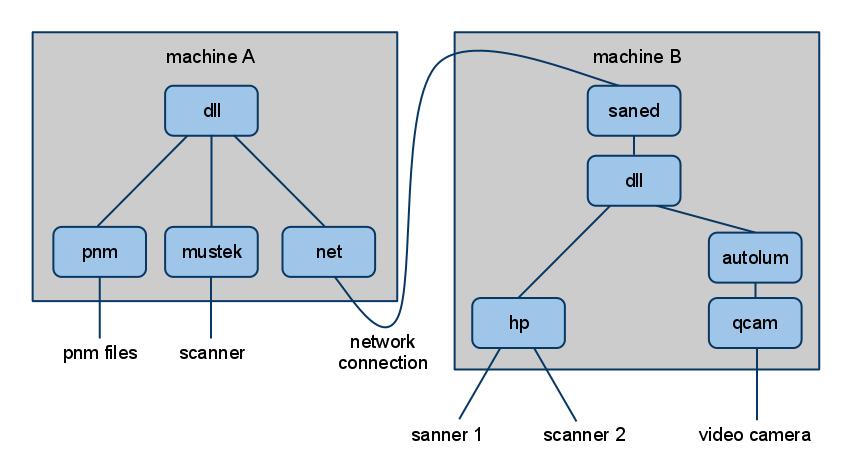
\includegraphics[height=0.5\hsize] {image201012/libsane02.png}
 \caption{SANEの構造}
\label{fig:sane}
\end{center}
\end{figure}

なお、
SANEを利用するユーザはscannerグループに所属させる必要があります。

\newpage

\subsection{Code Flow}

\begin{figure}[H]
\begin{center}
 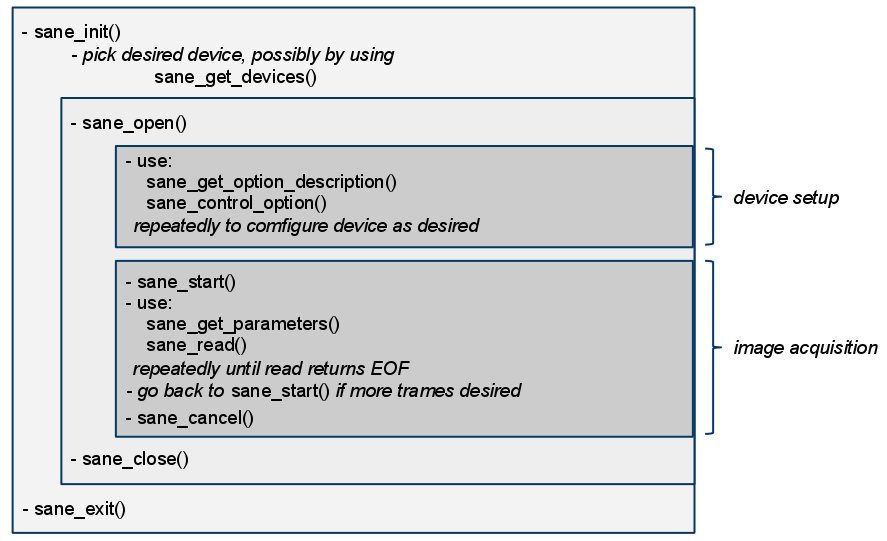
\includegraphics[height=0.5\hsize] {image201012/codeflow.png}
 \caption{Code Flow}
\label{fig:codeflow}
\end{center}
\end{figure}


\subsection{スキャンするためのコード}

とりあえずスキャンするだけのコードは次のようになります。

\begin{commandline}
#include <stdio.h>
#include <stdlib.h>
#include <string.h>

#include <sane/sane.h>


#define MAXLEN 32768

int main()
{
  SANE_Status stat;
  SANE_Handle hndl;
  SANE_Byte buf[MAXLEN];
  SANE_Int len = MAXLEN;
  FILE *fp;

  stat = sane_init(NULL, NULL);
  printf("init: %d\n", stat);
  stat = sane_open("fujitsu:libusb:008:002", &hndl);
  printf("open: %d\n", stat);

  fp = fopen("foo.bin", "wb");
  stat = sane_start(hndl);
  printf("start: %d\n", stat);
  while (len == MAXLEN) {
    stat = sane_read(hndl, buf, MAXLEN, &len);
    printf("read: %d\n", stat);
    printf("read_len: %d\n", len);
    fwrite(buf, len, 1, fp);
  }
  fclose(fp);

  sane_close(hndl);
  printf("close: %d\n", stat);
  sane_exit();
  printf("exit: %d\n", stat);
}
\end{commandline}

このコードで保存されるfoo.binは、
ScanSnap S1500の場合、
ヘッダ無しのpbmファイルとして保存されました。
スキャナによってはpgmで保存されるものもあり、
デフォルトで保存される画像のモードは特に決まっていないようです。


\subsection{カラーのスキャン}

オプションの設定にはいくつか注意点があるようです。

\begin{itemize}
\item sane\_get\_option\_descriptor()でオプションの説明文やフォーマットの取得が可能。
\item sane\_control\_option(hndl, 0, SANE\_ACTION\_GET\_VALUE, \&num, \&info)でオプションの総数を取得できる。
\item sane\_control\_option()でActionにSANE\_ACTION\_GET\_VALUEを指定することで現在設定されているオプションを読み出すことが可能。
\item sane\_control\_option()でActionにSANE\_ACTION\_SET\_VALUEを指定することでオプションの設定が可能。
\item sane\_control\_option()を呼ぶ際には事前にsane\_get\_option\_descriptor()を呼び出しておく必要がある。 
\end{itemize}

\begin{commandline}
#include <stdio.h>
#include <stdlib.h>
#include <string.h>
#include <sane/sane.h>

#define MAXLEN 32768

int main()
{
  SANE_Status stat;
  SANE_Handle hndl;
  const SANE_Option_Descriptor *opt;
  SANE_Int info = 0;
  SANE_Byte buf[MAXLEN];
  SANE_Int len = MAXLEN;
  SANE_Parameters param;
  FILE *fp;

  stat = sane_init(NULL, NULL);
  printf("stat: %d\n", stat);
  stat = sane_open("fujitsu:libusb:008:004", &hndl);
  printf("open: %d\n", stat);

  int x=300, y=300;
  opt = sane_get_option_descriptor(hndl, 4);
  printf("get_option_descriptor: %03d: %d\n", 0, opt->size);
  stat = sane_control_option(hndl, 4, SANE_ACTION_SET_VALUE, &x, &info);
  printf("control_option: %d\n", stat);
  printf("info: %d\n", info);

  opt = sane_get_option_descriptor(hndl, 5);
  printf("get_option_descriptor: %03d: %d\n", 0, opt->size);
  stat = sane_control_option(hndl, 5, SANE_ACTION_SET_VALUE, &y, &info);
  printf("control_option: %d\n", stat);
  printf("info: %d\n", info);

  strcpy(buf, "Color");
  opt = sane_get_option_descriptor(hndl, 3);
  printf("get_option_descriptor: %03d: %d\n", 0, opt->size);
  stat = sane_control_option(hndl, 3, SANE_ACTION_SET_VALUE, buf, &info);
  printf("control_option: %d\n", stat);
  printf("info: %d\n", info);

  stat = sane_start(hndl);
  printf("%d\n", stat);
  fp = fopen("foo.ppm", "wb");

  stat = sane_get_parameters(hndl, &param);
  printf("get_parameters: %d\n", stat);
  sprintf(buf, "P6\x0a# SANE data follows\x0a%d %d\x0a%d\x0a",
    param.pixels_per_line, param.lines, 255);
  fwrite(buf, strlen(buf), 1, fp);


  while (len == MAXLEN) {
    stat = sane_read(hndl, buf, MAXLEN, &len);
    printf("read: %d\n", stat);
    printf("read_len: %d\n", len);
    fwrite(buf, len, 1, fp);
  }
  fclose(fp);

  sane_close(hndl);
  printf("close: %d\n", stat);
  sane_exit();
  printf("exit: %d\n", stat);
}
\end{commandline}


\begin{figure}[H]
\begin{center}
 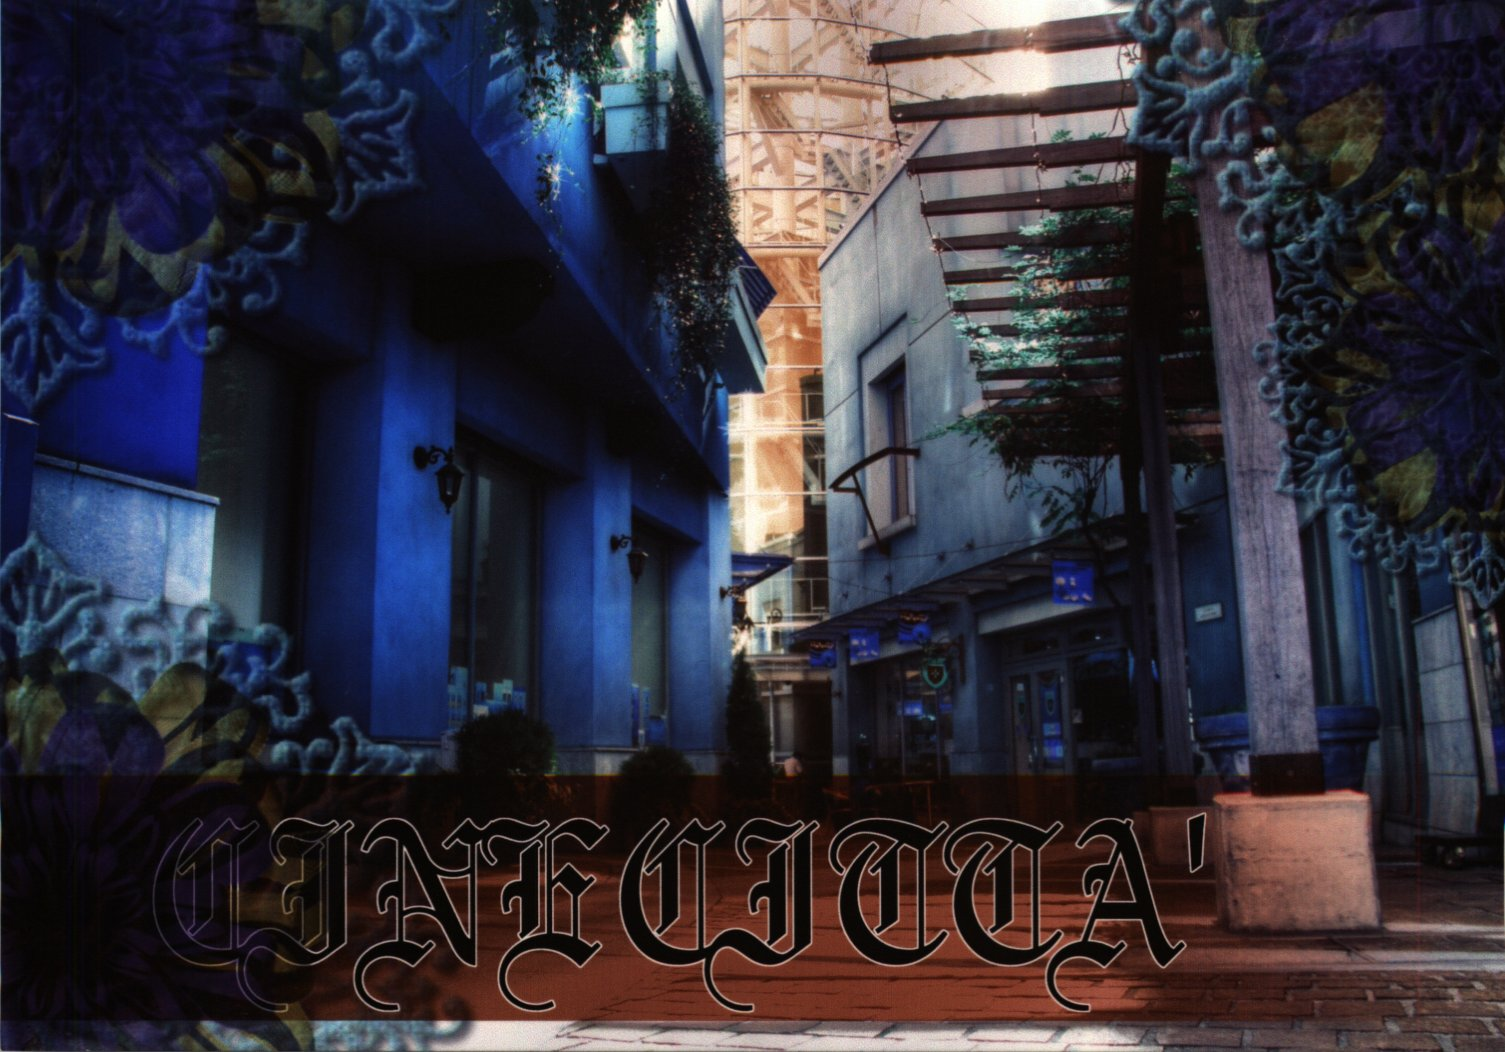
\includegraphics[height=0.5\hsize] {image201012/dst02.jpg}
 \caption{スキャン結果}
\label{fig:scan}
\end{center}
\end{figure}

モノクロではわかりづらいと思いますが、
ScanSnap S1500でスキャンした結果、
RとBが入れ替わってスキャンされました。

\subsection{まとめ}

\begin{itemize}
\item やや不安定(特に権限周り)
  \begin{itemize}
  \item scanimage -Lでたまにsegmentation faultする 
  \end{itemize}
\item スキャナによってデフォルトの動作がまちまち
  \begin{itemize}
  \item ScanSnapは.pbmでスキャン
  \item CanoScanは.pgmでスキャン 
  \end{itemize}
\item スキャナによってRGBの順番すらまちまち
  \begin{itemize}
    \item でもこれはScanSnapが悪いのかも
    \item ScanSnapはTWAIN未対応だし 
  \end{itemize}
\item ドキュメント化されていない罠の存在
\item スキャナのボタンをイベントとして使えないっぽい 
\end{itemize}

\begin{thebibliography}{0}
 \bibitem{sane}SANE - Scanner Access Now Easy \\
http://www.sane-project.org/

 \bibitem{sanejp}
SANE-tutorial-JP / 著者:David Mosberger / 翻訳:川岸 良治\\
http://archive.linux.or.jp/JF/JFdocs/SANE-tutorial-JP.html

 \bibitem{saneapi}
SANE Standard Version 2.0 proposal 0.08 - rauch/beck \\
http://www.sane-project.org/sane2/0.08/

\end{thebibliography}


\printindex

\cleartooddpage

\vspace*{15cm}
\hrule
\vspace{2mm}

\includegraphics[width=2cm]{image200502/openlogo-nd.eps}
\noindent \Large \bf Debian 勉強会資料\\
\noindent \normalfont \debmtgyear{}年\debmtgmonth{}月\debmtgdate{}日 \hspace{5mm}  初版第1刷発行\\
\noindent \normalfont 東京エリア Debian 勉強会 (編集・印刷・発行)\\
\hrule

\end{document}
